%!TEX root = ../dokumentation.tex

\chapter{Validierung}

\section{Vorgehensweise}
	\subsection{Nutzung von Starexec und TPTP}
		Zur Validierung der Arbeit werden Performancetests durchgeführt, die die Effizienz verschiedener Strategien vergleichbar machen.	Die Beweissuche wird auf der Hardware von Starexec durchgeführt, um eine möglichst konstante Rechenleistung zu haben. Wie in Sektion \ref{section:2StarexecTPTP} beschrieben, setzt sich ein Job aus einer Menge von Beweiser-Konfigurationen und einer Menge von Problemen zusammen. 
		
		Der verwendete Beweiser ist eine ZIP-Datei mit den Python-Dateien von PyRes. Er enthält die fertige Implementierung der SOS-Strategien. Konfigurationen sind ebenfalls in der ZIP-Datei enthalten und werden durch ein Text-Datei spezifiziert. Die Datei enthält den Befehl zum Ausführen von PyRes mit angegebenen Eingabeparametern. Diese Parameter geben vor, welche Optimierungen durchgeführt werden, beispielsweise Literalselektion, SOS-Strategie, SOS-Ratio usw.
		
		Die Probleme, auf die die Beweissuche angewandt wird, kommen von TPTP, einem Benchmark, der sich aus etwa 24000 Problemdateien zusammensetzt (siehe Sektion \ref{section:2StarexecTPTP}.
		
		Bei der Konfiguration eines Starexec-Jobs kann eine	maximale Rechenzeit angegeben werden, die ein Paar aus Problem und Konfiguration zugewiesen bekommt. Findet PyRes innerhalb dieser Zeit keine Lösung für das Problem, wird die Suche abgebrochen. Für alle Jobs sollte die maximale Rechenzeit gleich festgelegt sein, um die Starexec-Ergebnisse mehrerer Jobs vergleichbar zu machen. Der Standard-Wert bei Starexec liegt bei 300 Sekunden, der genaue Wert wurde für diese Arbeit auf 20 Sekunden herabgesetzt.
		
		Eine geringere Rechenzeit führt zwar zu weniger gelösten Problemen, aber die Jobs nehmen weniger Zeit in Anspruch. Da die Anzahl der gelösten Probleme in Abhängigkeit zur Zeit weniger als linear zunimmt, kann man davon ausgehen, dass es nur wenig Beweise gibt, die nach 20 Sekunden noch gefunden werden. Aus diesem Grund wurde der Vorteil der schnelleren Berechnungszeit höher gewichtet.
	
	\subsection{Zu analysierende Konfigurationen}
		Es wurden 3 SOS-Strategien implementiert und es gibt die Möglichkeit keine SOS-Strategie einzusetzen. Diese vier Möglichkeiten lassen sich mit Konzept 1 oder mit Konzept 2 kombinieren und können jeweils mit oder ohne Literalselektion durchgeführt werden. In der Theorie ergeben sich damit 16 Kombinationen, von denen nicht alle vollständig sind und es redundante Konfigurationen gibt. Folgende Tabelle zeigt eine Übersicht mit den möglichen Konfigurationen (siehe Tabelle \ref{table:possibleConfigs}). 		
		
		Wenn keine SOS-Strategie angegeben wird, dann erstellt PyRes standardmäßig ein Objekt der Klasse NoSos als Platzhalter (siehe Sektion \ref{section:4.1}). Für die Konfiguration ohne SOS sind Konzept 1 und 2 gleichbedeutend, da in beiden Fällen keine Klausel als Teil des SOS markiert wird und auch keine Klausel anfangs in die verarbeitete Klauselmenge einsortiert wird. Die Beweissuche ist mit und ohne Literalselektion vollständig.
		
		Die drei SOS-Strategien können mit beiden Konzepten kombiniert werden, allerdings ist Konzept 1 in Verbindung mit Literalselektion unvollständig. In Konzept 2 kann mit der Option "R" zusätzlich ein ganzzahliges Verhältnis angegeben werden, das die Verarbeitung von SOS und Nicht-SOS-Klauseln bestimmt. Für die Wahl dieses Wertes wurde sich für eine logarithmische Abstufung entschieden, da sie einen größeren Wertebereich abdeckt.
		
		
		\begin{table}[h]
			\centering
			\begin{tabular}{|c|c|c|c|c|c|}
				\hline
				& & \multicolumn{2}{c|}{SOS-Konzept 1} & \multicolumn{2}{c|}{SOS-Konzept 2} \\
				& & \multicolumn{2}{c|}{(Nicht-SOS $\rightarrow$ processed)} & \multicolumn{2}{c|}{(Priorisierte Verarbeitung)}  \\
				\cline{3-6}
				& & keine Literalsel. & Literalsel. & keine Literalsel. & Literalsel. \\
				\hline\hline
				 \multirow{4}{*}{\rotatebox[origin=c]{90}{SOS-Strategie}} & NoSos & \checkmark & \checkmark & redundant & redundant \\
				\cline{2-6}
				& Conjecture & \checkmark & unvolls. & \checkmark & \checkmark \\
				\cline{2-6}
				& OnlyPosLit & \checkmark & unvolls. & \checkmark & \checkmark \\
				\cline{2-6}
				& OnlyNegLit & \checkmark & unvolls. & \checkmark & \checkmark \\
				\hline
			\end{tabular}
			\label{table:possibleConfigs}
			\caption{Mögliche Konfigurationen für Performancetests. Unvollständige und redundante Konfigurationen werden nicht durchgeführt. Bei Konzept 2 kann die Konfiguration zusätzlich mit dem Verhältnis $R$ variiert werden.}
		\end{table}

	
	\subsection{Zu analysierende Größen}
	
	Wenn PyRes ein Problem innerhalb der angegebenen Zeit lösen kann, gibt es den bewiesenen Status des Problems in einer Ergebnisdatei aus. Des weiteren werden Informationen über die Beweissuche ausgegeben, zum Beispiel die Anzahl der berechneten Resolventen und die Zeit, die für die Beweissuche benötigt wurde.
	
	Folgende Größen können zur Performance-Analyse herangezogen werden.
	\begin{itemize}
		\item Die Anzahl der insgesamt gelösten Probleme von allen etwa 24000 TPTP Problemen macht eine Aussage über die Effizienz einer Konfiguration. Zusätzlich kann zwischen dem Status der Probleme (Erfüllbarkeit / Unerfüllbarkeit) differenziert werden, da eine Konfiguration, die schneller einen Widerspruch findet, nicht zwangsweise schneller die Erfüllbarkeit belegt.
		
		\item Die benötigte Zeit der gelösten Probleme kann zur Analyse herangezogen werden. Es kann sowohl die durchschnitte Zeit aller gelösten Probleme betrachtet werden, als auch der Graph, der den Verlauf der gelösten Probleme in Abhängigkeit zu Zeit darstellt.
		
		Da es vorkommt, dass zwei Konfigurationen nicht exakt die gleichen Probleme lösen, kann der Vergleich zwischen den Rechenzeiten verfälscht werden. Eine effizientere Konfiguration könnte beispielsweise viele Probleme schneller lösen, als eine ineffizientere Konfiguration. Die effizientere Konfiguration würde auch schwierige Probleme lösen, die die ineffizientere nicht löst. Auf diese Weise wird die durchschnittlich benötigte Rechenzeit der effizienten Konfiguration durch die hohe Rechnezeit der schwierigeren Probleme nach unten gezogen.
		
		Eine Lösung dafür ist, nicht alle gelösten Probleme in die Analyse einfließen zu lassen, sondern nur die Schnittmenge der gelösten Probleme unter allen Konfigurationen.
		
		\item Neben der Rechenzeit können die anderen Ergebnisgrößen wie berechnete Resolventen, berechnete Faktoren berücksichtigt werden. Auch hier sollten zum Vergleich zweier Konfigurationen lediglich die Probleme betrachtet werden, die unter allen Konfigurationen gelöst werden.
		
		\item Eine weitere Möglichkeit, zwei Konfigurationen zu vergleichen, ist, die Probleme im direkten Vergleich in Bezug zu setzen. Anstatt wie oben genannt, alle Rechenzeiten einer Konfiguration mit allen Rechenzeiten der anderen Konfigurationen zu vergleichen, werden für jedes Problem einzeln die Rechenzeiten verglichen. Somit kann für jedes einzelne Problem eine prozentualer Abweichung errechnet werden. Über alle Probleme kann dann ein Mittelwert gebildet werden.
	\end{itemize}
	Es ist davon auszugehen, dass die betrachteten Größen stark korrelieren. Eine Konfiguration, die mehr Probleme als eine andere löst, wird die meisten Probleme auch schneller lösen und mit weniger berechneten Resolventen.
	
	\subsection{Prüfung widersprüchlicher Ergebnisse}
		Für alle StarExec-Ergebnisse kann geprüft werden, ob Widersprüche zwischen dem gefundenen Status und dem tatsächlichen Status vorliegen, da in jedem Problem der tatsächliche Status des Problems angegeben ist. ob  Ein Widerspruch liegt dann vor, wenn ein Problem in einer Konfiguration als unerfüllbar eingestuft wurde, aber in Wirklichkeit erfüllbar ist, oder vice versa. In solch einem Fall ist der Beweiser fehlerhaft, vorausgesetzt der angegebene tatsächliche Status ist korrekt. Alle Ergebnisse dieses Kapitels wurden geprüft und sind widerspruchsfrei.

\section{Ergebnisse}
	\subsection{Vergleich der SOS-Strategien}
	\label{section:vglSOS}
		\paragraph{Vergleich nach Anzahl gelöster Probleme}
		
	 	Um die drei SOS-Strategien zu vergleichen, werden die Ergebnisse ohne SOS-Strategie als Referenzwerte herangezogen.
	 	Es ist davon auszugehen, dass die Rangfolge der Strategien unter Konzept 1 und Konzept 2 gleich ist, da sich die Einteilung der Klauseln nicht unterscheidet und die Abarbeitung der Klauseln nur geringfügig angepasst wird. Aus diesem Grund wird vorerst nur Konzept 1 analysiert.
	 	\begin{figure}
	 		\centering
	 		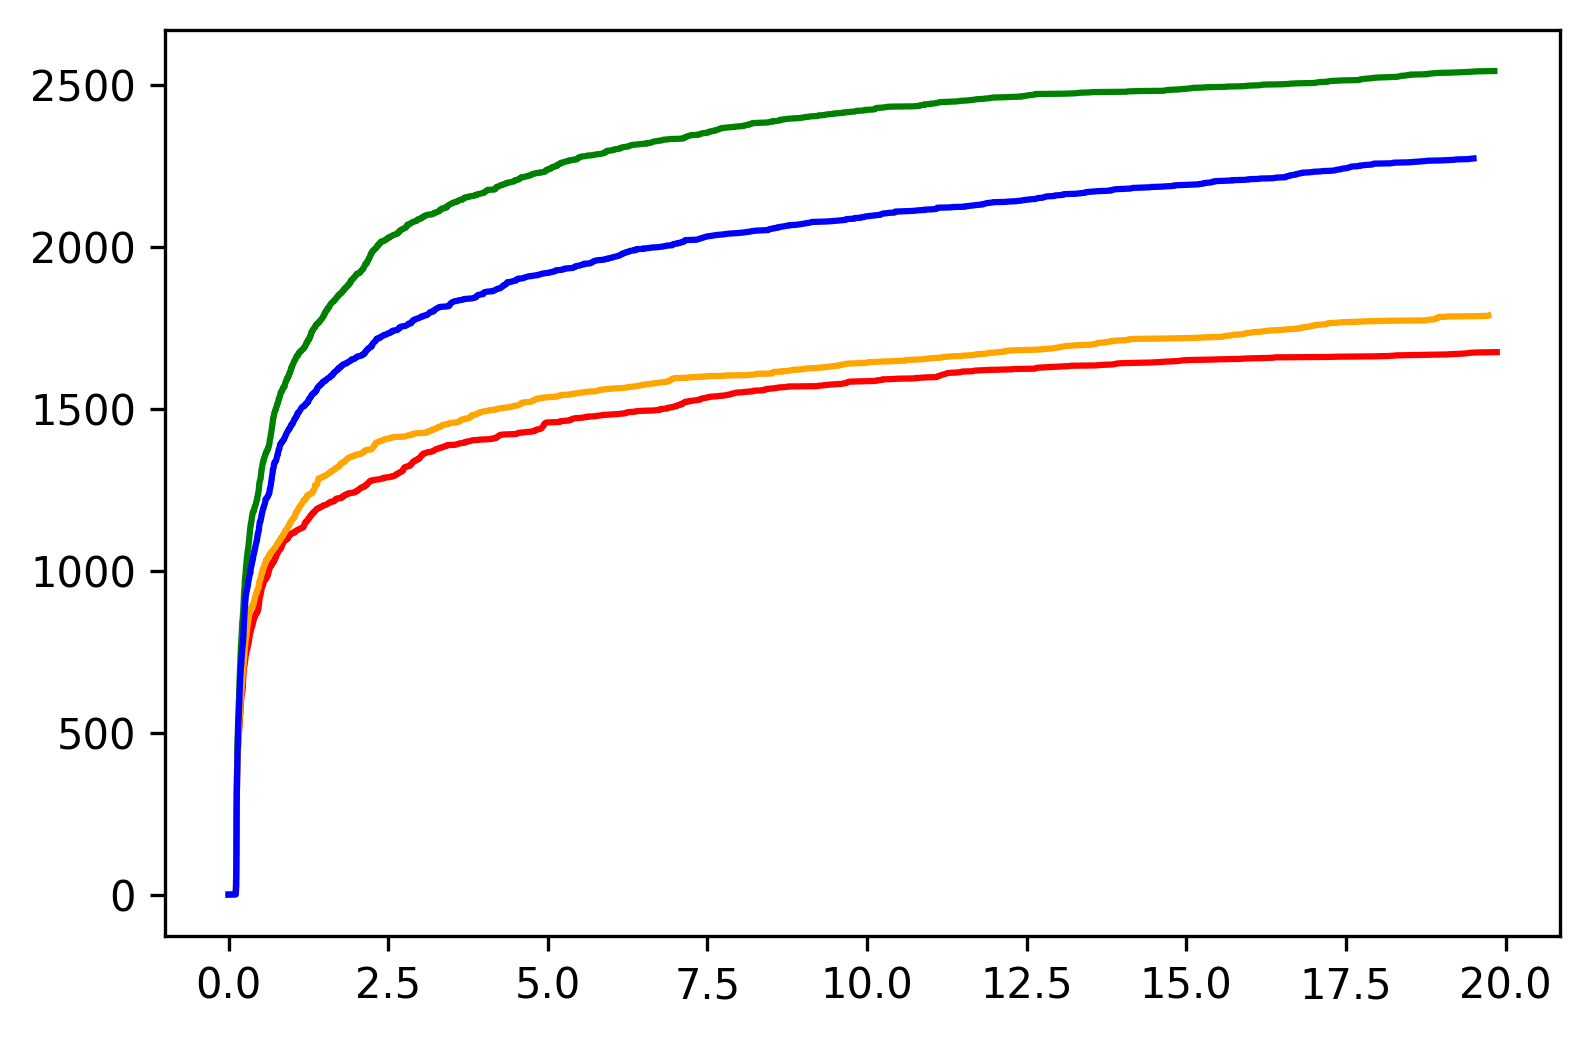
\includegraphics[width=0.45\linewidth]{images/Diagram/time_comapre}
	 		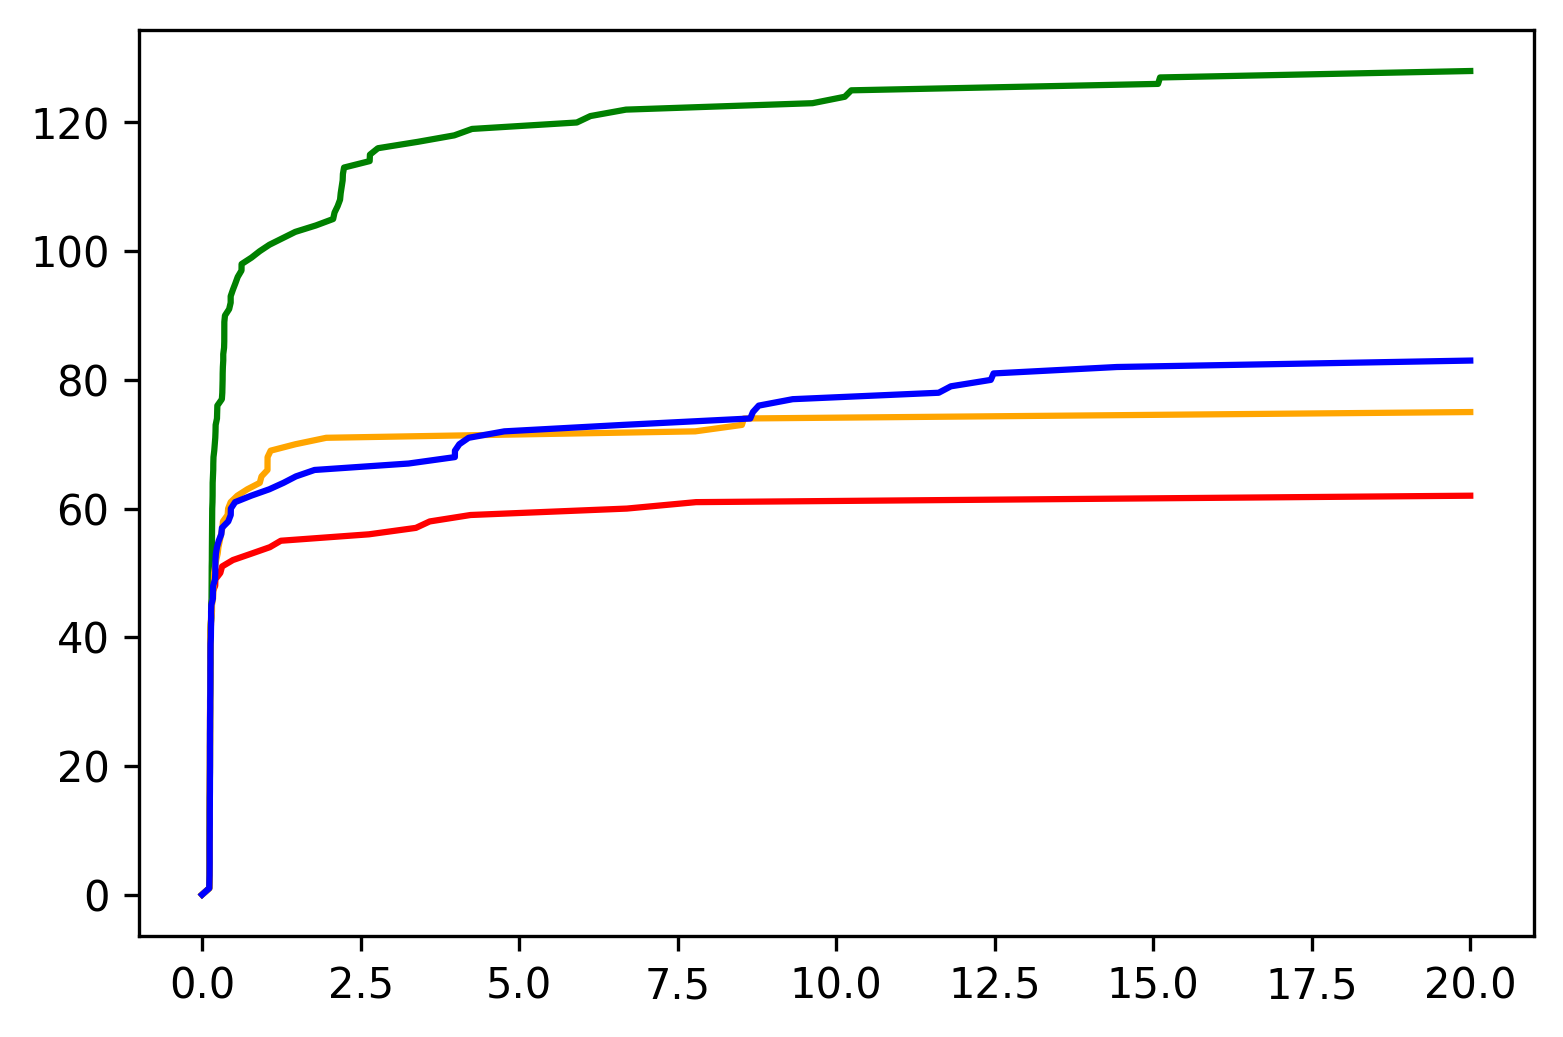
\includegraphics[width=0.45\linewidth]{images/Diagram/time_comapre2}
	 		\caption{Anzahl der gelösten Probleme nach der Zeit für die vier betrachteten Konfigurationen. Links: alle gelösten Probleme, Rechts: erfüllbare gelöste Probleme, Rot: kein SOS, Grün: Vermutung als SOS, Orange: rein positive Literale als SOS, Blau: rein negative Literale als SOS}
	 		\label{fig:timecomapre}
	 	\end{figure}
	 	
	 	Die Anzahl der gelösten Probleme deutet darauf hin, dass alle drei SOS-Strategien besser sind, als keine SOS-Strategie. (siehe Abbildung \ref{fig:timecomapre})
	 	Ein Grund dafür könnte sein, dass in jeder zugelassenen SOS-Strategie Kombinationen für die Resolution verboten werden, vorausgesetzt die Menge der Nicht-SOS-Klauseln enthält mehr als eine Klausel. Da Grundklauselmenge stets erfüllbar ist, tragen diese Kombinationen nichts zur Beweissuche bei.
	 	
	 	Mit Abstand am besten schneidet Strategie 1 ab, welche die negierte Vermutung in das SOS steckt. Sie löste 2544 Probleme, im Vergleich zu 1676 ohne SOS. Eine Grund dafür könnte sein, dass der Beweis eher vom Ziel ausgeht und somit eher in Richtung des Widerspruchs geleitet wird. Meistens ist die Menge der Vermutungsklauseln geringer, als die Menge der Axiome. Somit wird ein großer Teil irrelevanter Kombinationen vermieden.
		
		Strategie 3 (OnlyPosLit) ordnet rein positive Klauseln dem SOS zu schneidet als zweitbestes ab und löst mit 2273 Problemen deutlich mehr als Strategie 2 (OnlyNegLit) mit 1788. Syntaktisch gesehen, sind beide Strategien gleichwertig, da sich die Erfüllbarkeit durch Negieren aller Literale nicht verändert. Der Grund für die starken Unterschiede muss demnach auf der semantischen Ebene liegen und mit den Bedeutungen der Klauseln und zusammenhängen. 
		
		Eine Vermutung ist, dass Axiome tendenziell häufiger positiv formuliert werden und dadurch viele positiven Literale enthalten. Da Vermutungen negiert werden, um einen Widerspruch zu erzeugen, könnte es bei ihnen häufiger vorkommen, dass sie unter Strategie 3 ins SOS sortiert werden. Wie schon an Strategie 1 ersichtlich ist, bietet das Zuweisen der Vermutungen zum SOS einen signifikanten Vorteil.
	
		Weiterhin kann aus Abbildung \ref{fig:timecomapre} gelesen werden, dass nicht nur bei unerfüllbaren Problemen schneller ein Widerspruch gefunden wird, sondern auch, dass die Erfüllbarkeit von Problemen schneller bewiesen werden kann. Allerdings ist die Menge dieser Probleme so gering, dass genau Zahlenwerte sehr unsicher sind. Das kann man unter anderem daran erkennen, dass der Verlauf der Linien ungleichmäßig ist.
	
		\paragraph{Vergleich der Schnittmengen zwischen den Strategien}
	
		Betrachtet man die Menge der gelösten Probleme und deren Schnittmengen, sieht man, dass es teilweise große Überlappungen zwischen den gelösten Problemen gibt. (siehe Tabelle \ref{table:geloestSchnittmenge}, Abbildung \ref{fig:venn2} und Abbildung \ref{fig:venn3} Fast alle Probleme, die ohne SOS gelöst wurden, wurden auch mit einer beliebigen SOS-Strategie gelöst. 
		Von den 1676 Problemen, die ohne SOS gelöst wurden, löste SOS-Strategie 1 1620 Probleme. Nur 56 Probleme, also 3,3 \% konnten nicht von SOS-Strategie 1 gelöst werden. Dieses Ergebnis kann als positiv angesehen werden, da es nur wenig Fälle gibt, in denen SOS einen Nachteil bringt.
	
		Auch die Schnittmenge aller drei SOS-Strategien ist relativ hoch. Von den 1788 Probleme, die die schlechteste Strategie löst, werden 1633 Probleme von allen drei Strategien gelöst. (siehe Abbildung \ref{fig:venn3}, links) 
		
		Im mittleren Diagramm in Abbildung \ref{fig:venn3} werden nur diejenigen Probleme betrachtet, die auch ohne SOS gelöst wurden. Dies sind die tendenziell einfacheren Probleme. Anschaulich werden die drei Schnittmengen aus Abbildung \ref{fig:venn2} genommen und zu einem neuen Diagramm zusammengeführt. Man stellt fest, dass die Überlappung für dieses Diagramm noch größer wird. Die ist wenig überraschend, da bereits in Abbildung \ref{fig:venn2} zu sehen war, dass fast alle Probleme, die ohne SOS gelöst wurde, auch von den drei Strategien gelöst wird.
		
		Auf der rechten Seite von Abbildung \ref{fig:venn3} sind nur die Probleme dargestellt, die nicht von der Konfiguration ohne SOS gelöst wurden. Dies sind die tendenziell schwierigeren Probleme. Dieses Diagramm setzt sich also aus den drei rechten Teilmengen von Abbildung \ref{fig:venn2} zusammen.
		Auffällig ist hier, dass die Überschneidung der Probleme wesentlich geringer ist. Daraus kann geschlussfolgert werden, dass es sinnvoll sein kann, das gleiche Problem mit unterschiedlichen SOS-Strategien zu kombinieren. Anstatt einem Problem eine Rechenzeit von $t$ zuzuweisen, könnte man die Beweissuche $n$ mal mit der Rechenzeit $t/n$ durchführen und dabei $n$ getrennte Strategien anwenden.
	
	
		\begin{table}
			\centering
			\begin{tabular}{|c|c|c|c|c|}
				\hline
				& NoSos & Conjecture & OnlyPosLit & OnlyNegLit \\ \hline
				NoSos & \textbf{1676} & & & \\ \hline
				Conjecture & 1614 & \textbf{2544} & & \\ \hline
				OnlyPosLit & 1582 & 1697 & \textbf{1788} & \\ \hline
				OnlyNegLit & 1600 & 1992 & 1666 & \textbf{2273} \\ \hline
				
			\end{tabular}
			
			\caption{Die Elemente der Hauptdiagonalen geben an, wie viele Probleme mit einer Strategie gelöst wurden. Die restlichen Elemente geben die Anzahl der Probleme an, die von beiden Strategien gelöst wurden.}
			\label{table:geloestSchnittmenge}
		\end{table}
	
		\begin{figure}
			\centering
			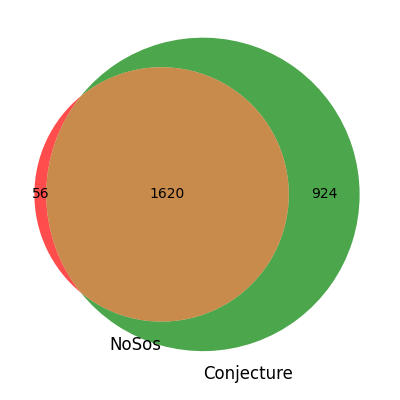
\includegraphics[width=0.3\linewidth]{images/Venn/venn2_sos1}
			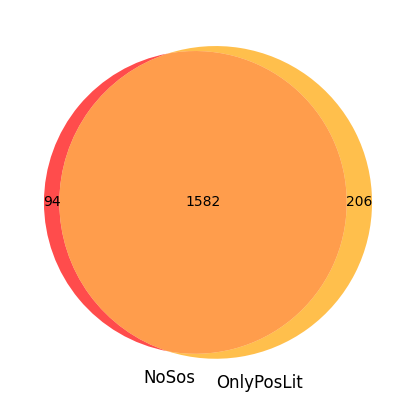
\includegraphics[width=0.3\linewidth]{images/Venn/venn2_sos2}
			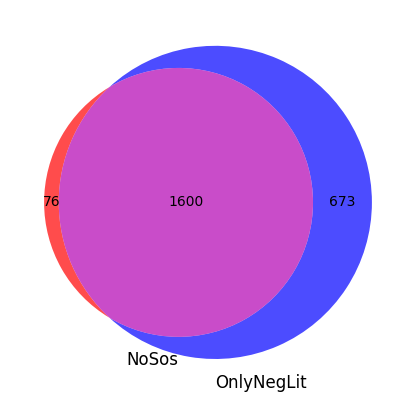
\includegraphics[width=0.3\linewidth]{images/Venn/venn2_sos3}
			\caption{Die drei Venn-Diagramme zeigen jeweils die gelösten Probleme einer SOS-Strategie im Vergleich zur Konfiguration ohne SOS.
			}
			\label{fig:venn2}
		\end{figure}
		
		\begin{figure}
			\centering
			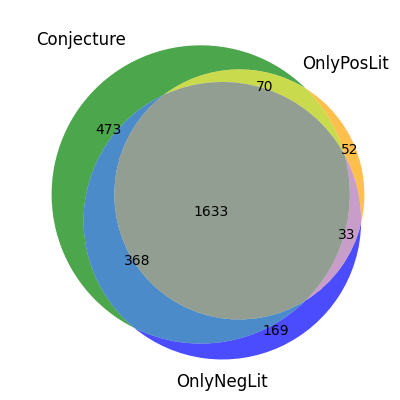
\includegraphics[width=0.3\linewidth]{images/Venn/venn3_both}
			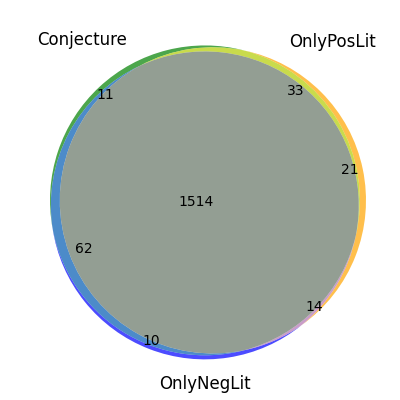
\includegraphics[width=0.3\linewidth]{images/Venn/venn3_solve}
			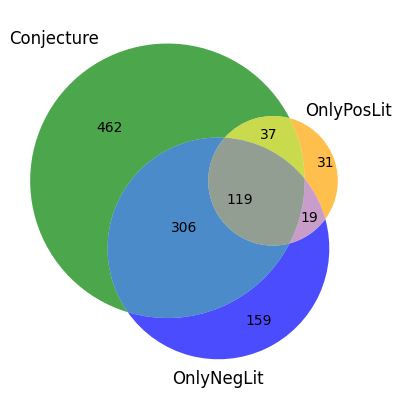
\includegraphics[width=0.3\linewidth]{images/Venn/venn3_notsolve}
			\caption{Die drei Venn-Diagramme zeigen die gelösten Probleme der drei SOS-Strategien im direkten Vergleich. Links sind alle gelösten Probleme zu sehen, in der Mitte nur die Probleme, die auch ohne SOS gelöst wurden und rechts nur die Probleme, die ohne SOS nicht gelöst wurden.
			Diese Darstellungsform wurde gewählt, da es nicht möglich ist, ein Venn-Diagramm aus 4 Mengen zu erstellen.}
			\label{fig:venn3}
		\end{figure}
		
		\paragraph{Vergleich nach Rechenzeit}
		Betrachtet man die 1620 Probleme, die sowohl ohne SOS als auch mit Strategie 1 gelöst wurden, und berechnet die durchschnittliche Rechenzeit, kommt man ohne SOS auf 1,8 Sekunden und mit SOS-Strategie 1 auf 0,9 Sekunden. Die durchschnittliche Rechenzeit kann als grober Richtwert verwendet werden, um zwei Konfigurationen zu vergleichen. Da der Zusammenhang zwischen gelösten Problemen und der Zeit nicht linear ist, kann aber nicht geschlussfolgert werden, dass eine Konfiguration mit SOS-Strategie 1 ein Problem im Mittel doppelt so schnell löst wie eine Konfiguration ohne SOS.
		
		Stattdessen wird für jedes Problem, das für beide Konfigurationen gelöst wurde, der Quotient der Rechenzeiten berechnet. Ein Wert von 0.5 bedeutet, dass die Konfiguration mit Strategie 1 doppelt so schnell war als die ohne SOS. Ein Wert von 2 bedeutet, dass die Berechnung ohne SOS doppelt so schnell war. Diese Größen werden logarithmiert, um die Berechnung des Durchschnitts zu ermöglichen. Würde man die Logarithmierung nicht vornehmen, würden die Werte 0,5 um 2 beim mitteln nicht 1 ergeben sondern 0,75. Die logarithmierten Größen werden gemittelt, anschließend wird die Logarithmierung durch die Exponentialfunktion rückgängig gemacht.
		
		Auf diese Weise stellt man fest, dass die Konfiguration mit SOS-Strategie 1 für ein Problem durchschnittlich nur 60 \% der Zeit benötigt, im Vergleich zu keiner SOS-Strategie. Strategie 2 benötigt 90 \% der Zeit und Strategie 3 69 \% der Zeit.
		
		
		Der Zusammenhang ist auch in Abbildung \ref{fig:directcompare} erkennbar. Jeder Datenpunkt ist ein Problem. Die x- bzw. y-Position zeigt die benötigte Zeit für jeweils eine der beiden Konfigurationen. Konnte ein Problem unter einer Konfiguration nicht gelöst werden, wird der Datenpunkt außerhalb der schwarzen Umrandung platziert. Im linken Diagramm lässt sich erkennen, dass fast jedes Problem, das von beiden Konfigurationen gelöst wurde, mit SOS-Strategie 1 schneller gelöst werden konnte.
		
		\begin{figure}
			\centering
			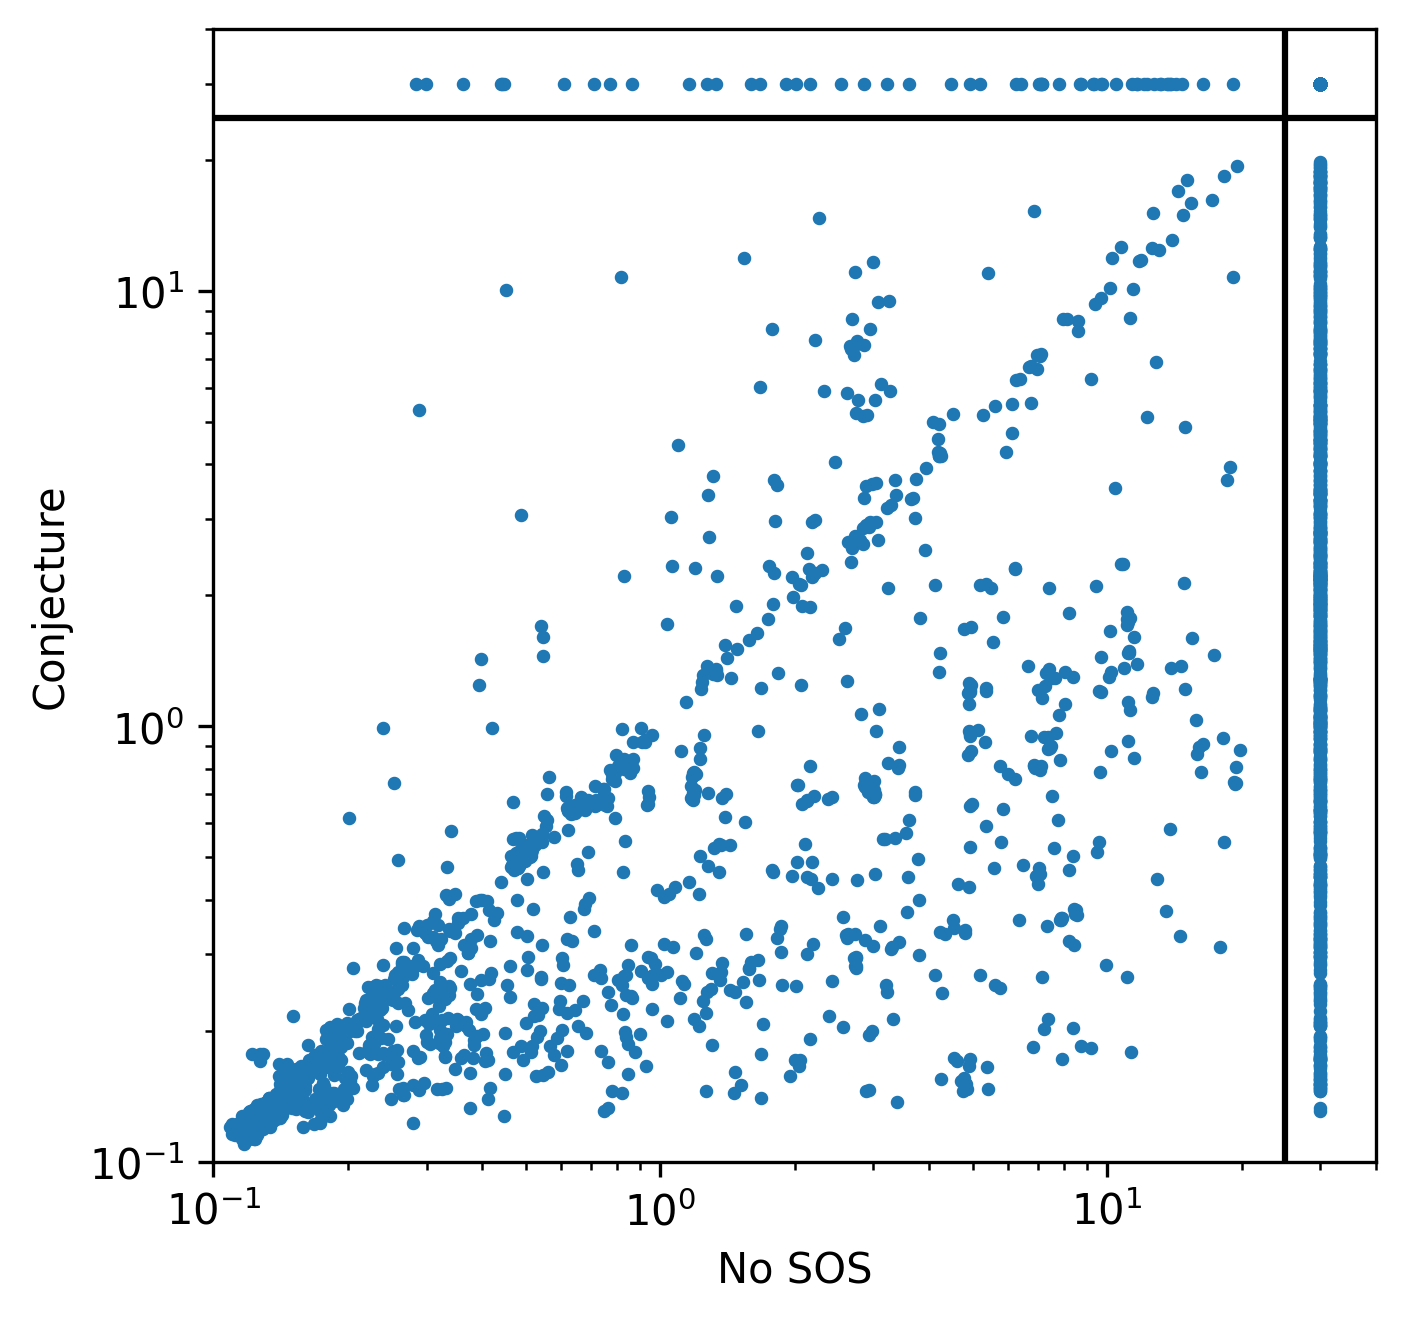
\includegraphics[width=0.45\linewidth]{images/Diagram/directCompare1_2}
			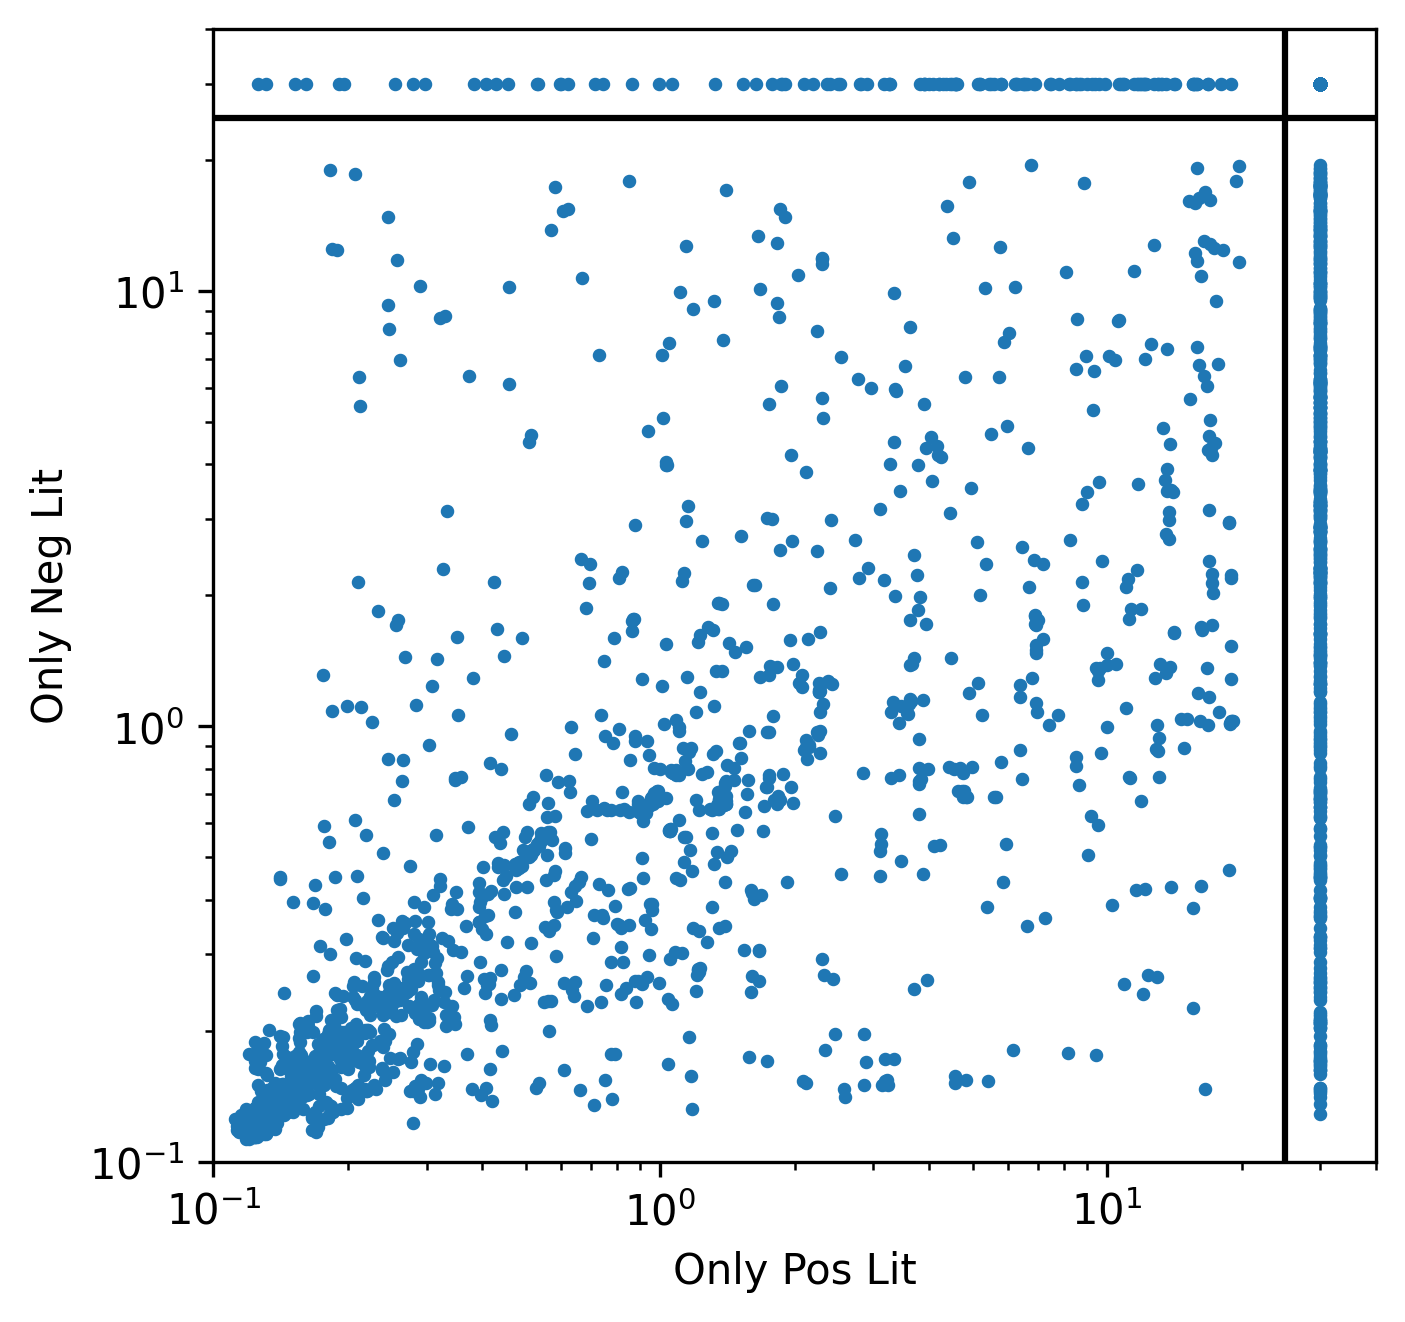
\includegraphics[width=0.45\linewidth]{images/Diagram/directCompare2_3}
			\caption{Benötigte Rechenzeit nach Problemen. Links: Vergleich zwischen NoSOS und Strategie 1, Rechts: Vergleich zwischen Strategie 2 und Strategie 3. Probleme, die von einem oder von beiden Konfigurationen nicht gelöst wurden, sind außerhalb des großen Quadrats dargestellt, um das Ergebnis nicht zu verfälschen.}
			\label{fig:directcompare}
		\end{figure}

		\paragraph{Betrachtung von Horn-Klauseln}
		Alle TPTP-Probleme enthalten in der .p-Datei verschiedene Tags, die Aussagen über die Eigenschaften des Problems machen. Einer dieser Tags ist die Information, ob eine Problem als Hornklauselmenge vorliegt oder nicht. Im Folgenden wird analysiert, ob die Effizienz von SOS davon abhängig ist, ob das Problem in Hornform vorliegt.
	
		Eine Hornformel ist eine prädikatenlogische Formel der Form
		$$A_1 \wedge A_2 \wedge \ldots \wedge A_n \rightarrow B$$
		$A_1$ bis $A_n$ sowie $B$ sind prädikatenlogische Atome und lassen sich in Klauselnormalform folgendermaßen darstellen.
		$$\{\neg A_1, \neg A_2, \ldots, \neg A_n, B\}$$
		Das Atom $B$ ist nicht zwingend notwendig und auch die Atome $A_1$ bis $A_n$ müssen nicht vorhanden sein. Allgemein ist eine Klausel eine Hornklausel, wenn sie maximal ein positives Literal enthält. \cite{Makowsky1987horn}
		Eine Klauselmenge ist genau dann eine Hornklauselmenge, wenn jede Klausel eine Hornklausel ist. Hornklauseln gelten in der Literatur als sehr elegant, da es viele Algorithmen gibt, mit denen Hornklauseln einfach und schnell verarbeitet werden können. \cite{Wild2017horn}
	
		Tabelle \ref{tab:Horn} zeigt, wie viele der Probleme in Hornform bzw. nicht in Hornform von den verschiedenen SOS-Strategien gelöst werden.
		Auffällig ist erstens, dass von den Hornproblemen ein viel größerer Anteil gelöst wird. Diese Tatsache ist unabhängig von der SOS-Strategie und ist deshalb nur auf die besseren Eigenschaften von Hornklauseln zurückzuführen.
		
		Zweitens fällt auf, dass die Anzahl der gelösten Probleme bei den Problemen in Hornform deutlich näher zusammenliegen, als bei den Problemen ohne Hornform. In beiden Fällen schlägt jede der drei SOS-Strategien die Konfiguration ohne SOS, doch der Unterschied ist in der rechten Spalte deutlich stärker vertreten. Ein Grund dafür könnte sein, dass die Probleme in Hornform einfacher zu lösen sind und SOS deshalb keinen so starken Vorteil bringt.
		\begin{table}
			\centering
			\begin{tabular}{|c|c|c|}
				\hline
				&Hornform & nicht Hornform \\
				\hline
				Anzahl Probleme & 1291 & 3949 \\
				\hline\hline
				NoSos & 402 & 288 \\
				\hline
				Conjecture & 498 & 647 \\
				\hline
				OnlyPosLit & 435 & 326 \\
				\hline
				OnlyNegLit & 526 & 486 \\
				\hline\hline
				Von allen gelöst & 379 & 246 \\ \hline
			\end{tabular}
		\caption{gelöste Probleme der SOS-Strategien geteilt in Horn- und Nicht-Horn-Probleme}
		\label{tab:Horn}
		\end{table}

	
	\subsection{Vergleich der beiden SOS-Konzepte}
	\label{sec:sos2}
	In der vorherigen Sektion konnte gezeigt werden, dass SOS-Strategien im Vergleich zur Beweissuche ohne SOS-Strategie einen Vorteil in der Effizienz bringen. Ein Nachteil ist, dass das bisher betrachtete Konzept 1, welches strikt vorgeht und nur SOS-Klauseln verarbeitet, nicht mit Literalselektion und geordneter Resolution kompatibel ist. Aus diesem Grund wurde ein zweites Konzept implementiert, welches in wählbaren Abständen $r$ Nicht-SOS-Klauseln verarbeitet. Dadurch bleibt die Vollständigkeit auch mit anderen Optimierungsstrategien vollständig.
	
	Der direkte Vergleich zwischen SOS-Konzept 1 und 2 wurde lediglich in Kombination mit SOS-Strategie 1 vorgenommen, da diese Strategie, wie bereits herausgefunden wurde, am effizientesten ist.
	
	Auf StarExec wurden Tests mit 10 Konfigurationen durchgeführt. Der Wert $r$ wurde zwischen 1 und 64 variiert. Ein Wert von 1 bedeutet, dass nach jeder SOS-Klausel eine Nicht-SOS-Klausel verarbeitet wird. Ein Wert von 64 bedeutet, dass erst 64 SOS-Klauseln verarbeitet werden und danach eine Nicht-SOS-Klausel. Das tatsächliche Verhältnis kann abweichen, da beim Nicht-Vorhandensein einer SOS-Klausel als nächstes eine Nicht-SOS-Klausel verarbeitet wird.
	
	Es ist erkennbar, dass die Effizienz für große und kleine Werte von $r$ etwas nach unten geht. Das Optimum liegt etwa im Bereich zwischen 2 und 4. Anzumerken ist, dass der Verlauf keine genaue Optimumskurve ergibt. Ein Grund dafür könnte sein, dass die Datenbasis zu gering ist und deshalb Abweichungen zustande kommen. Ein weiterer Grund könnte sein, dass für die Klauselauswahl nicht nur SOS entscheidend ist, sondern auch die angewandte Heuristik-Strategie. Die eingesetzte Strategie PickGiven5 wendet genau wie SOS ein Verhältnis an, das die Klauselauswahl beeinflusst. Je nachdem, wie die beiden Verhältnisse gewählt sind, könnte es zu Interferenzen kommen, die die Performance steigern oder mindern.
	
	Der maximale Wert an gelösten Klauseln konnte mit einem Wert von 4 für $r$ erzielt werden. Der Beweiser konnte mit dieser Konfiguration 2080 Probleme lösen. Mit Konzept 1 konnte ein Höchstwert von 2544 gelösten Probleme erreicht werden. Ohne weitere Optimierungen schneidet also Konzept 1 besser ab, als Konzept 2. In Konzept 2 steckt jedoch noch mehr Potenzial, da es mit negativer Literalselektion kombiniert werden kann. Die Ergebnisse dazu werden in der nächsten Sektion diskutiert.
	\begin{figure}
		\centering
		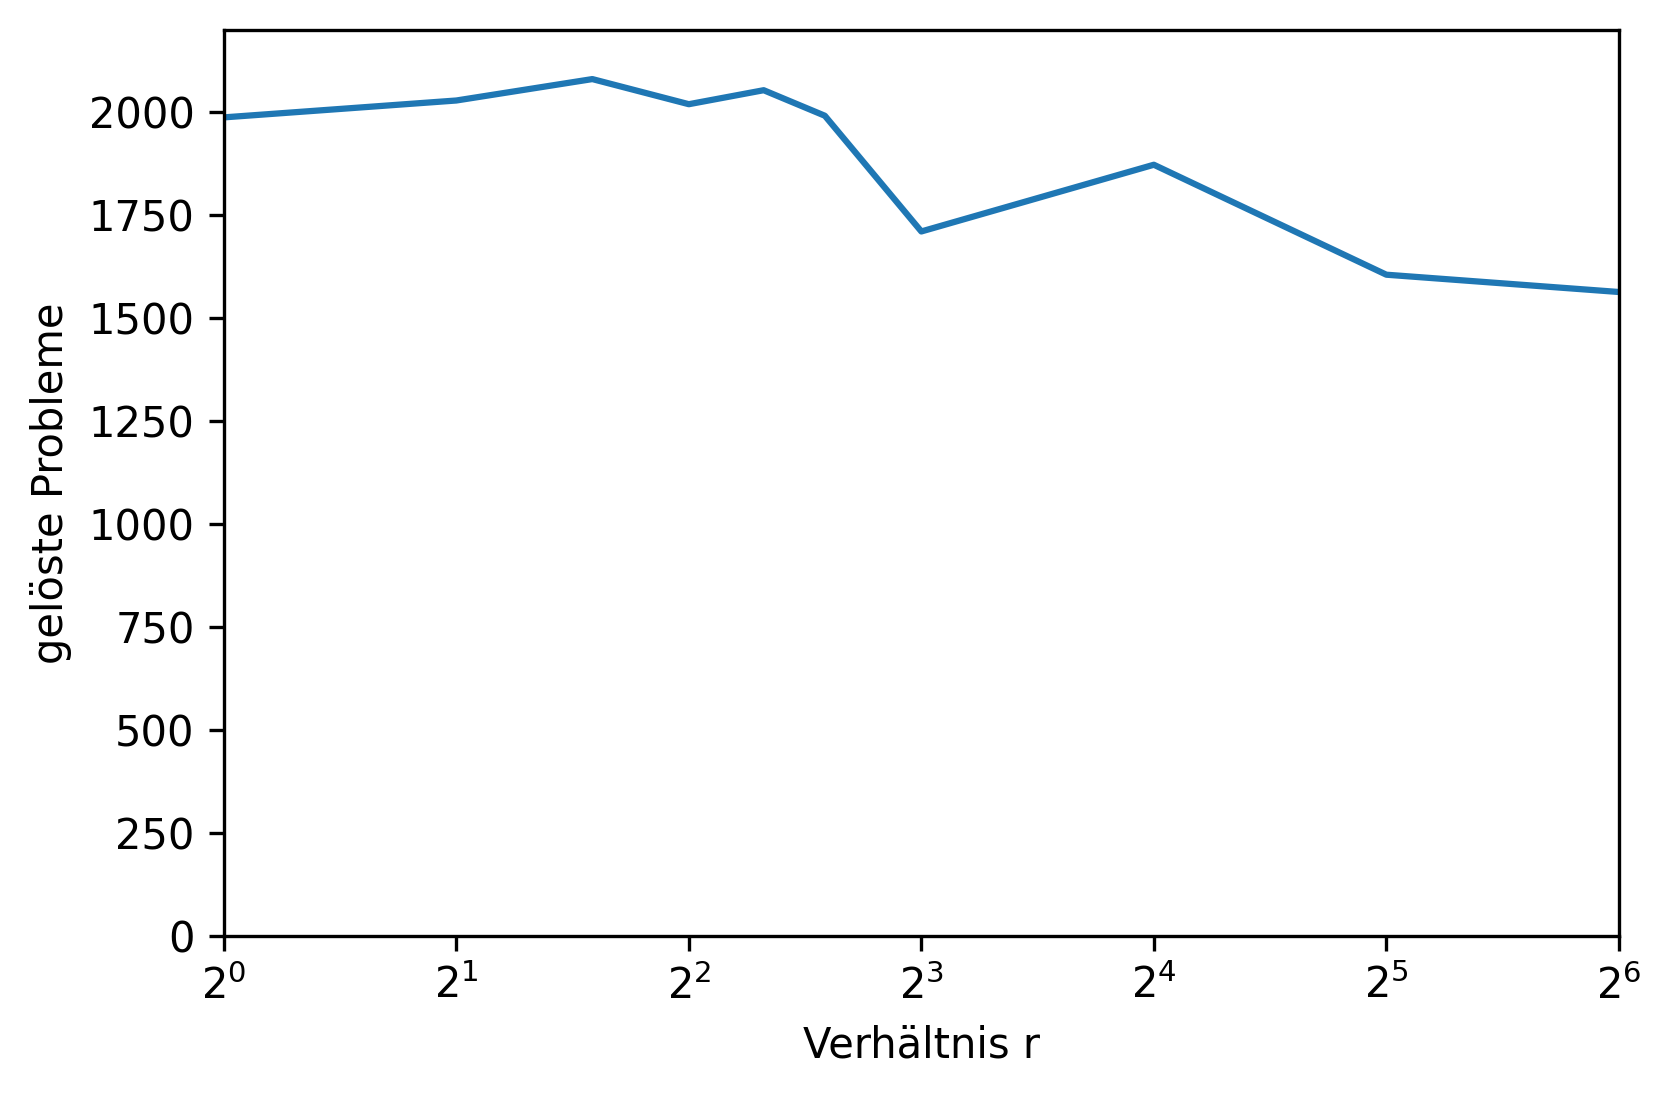
\includegraphics[width=0.45\linewidth]{images/Diagram/RWert}
		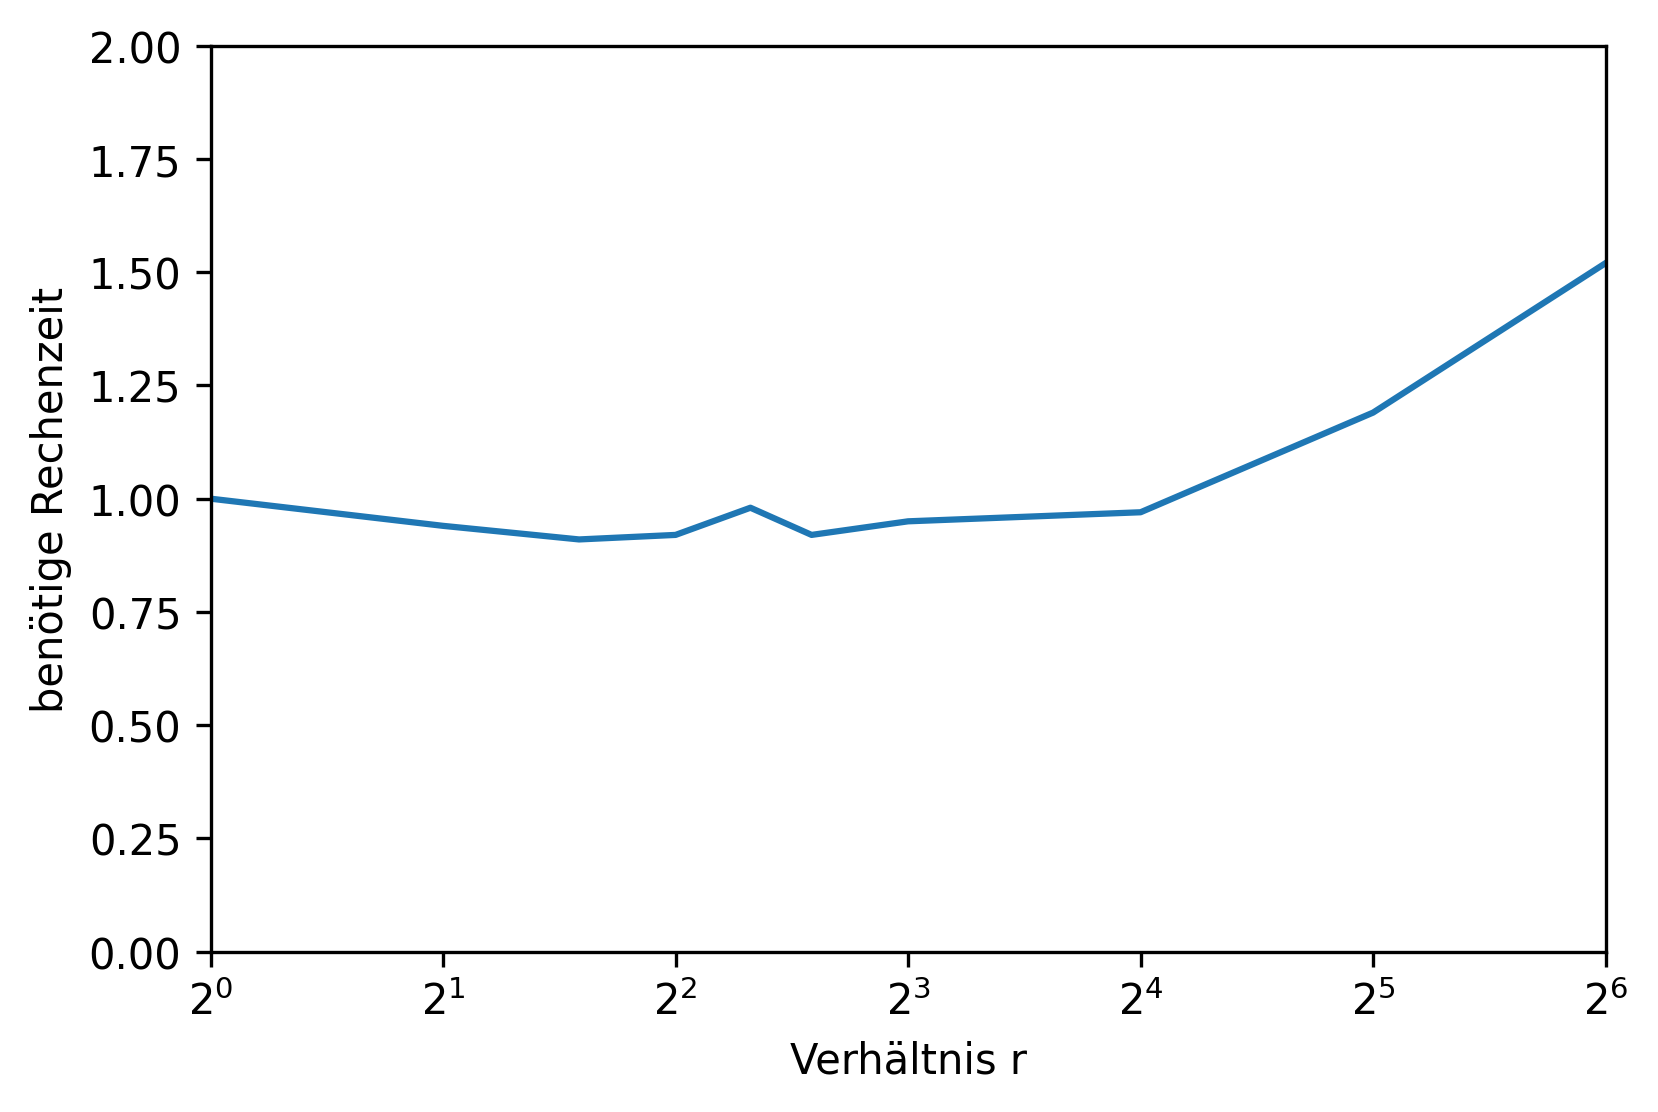
\includegraphics[width=0.45\linewidth]{images/Diagram/RWert2}
		\caption[Performance von Konzept 2 in Abhängigkeit von r]{Performance von Konzept 2 in Abhängigkeit von r. links: y-Achse zeigt die Anzahl der gelösten Probleme. rechts: y-Achse zeigt die durchschnittlich benötigte Rechenzeit für die Probleme, die von allen 7 Konfigurationen gelöst wurden.}
		\label{fig:rwert}
	\end{figure}
	
	
	\subsection{SOS-Strategie mit negativer Literalselektion}
	Wie gezeigt, schneidet SOS-Konzept 2 ohne weitere Optimierungen schlechter ab, als Konzept 1. Setzt man allerdings zusätzlich Literalselektion ein, werden mehr Probleme gelöst als mit Konzept 1.
	Für einen Wert für $r$ von 3, löst PyRes insgesamt 2880 Probleme. Dies ist der höchste Wert, die in dieser Arbeit erzielt wurde. 
	
	\begin{table}[h]
		\centering
		\begin{tabular}{|c|c|c|c|c|}
			\hline
			& \multicolumn{2}{c|}{SOS-Konzept 1} & \multicolumn{2}{c|}{SOS-Konzept 2} \\
			& \multicolumn{2}{c|}{(Nicht-SOS $\rightarrow$ processed)} & \multicolumn{2}{c|}{(Priorisierte Verarbeitung)}  \\
			\hline
			& keine Literalsel. & Literalsel. & keine Literalsel. & Literalsel. \\
			\hline\hline
			NoSos & 1676 & 2566 & redundant & redundant \\
			\hline
			Conjecture & 2544 & unvolls. & 2080 (r=4) & 2880 (r=3) \\
			\hline
		\end{tabular}
		\label{table:resultConfigs}
		\caption{gelöste Probleme bestimmten Konfigurationen. Bei SOS-Konzept 2 wurde jeweils die Konfiguration mit dem Wert $r$ ausgewählt, bei der die meisten Probleme gelöst wurden.}
	\end{table}
	
		
\section{Bewertung}
	\subsection{Nutzen von SOS}
	In den vorherigen Sektionen wurde die Performance verschiedener Konfigurationen mit SOS-Strategien analysiert. Im Folgenden werden die wichtigsten Ergebnisse zusammengefasst.
	
	Alle drei SOS-Strategie sind effizienter als eine Konfiguration ohne SOS-Strategie. Am besten schneidet Strategie 1 ab, welche die Vermutung als SOS wählt. 
	
	Von den beiden implementierten Konzepten schneidet Konzept 1 zwar besser ab. Konzept 2 kann jedoch mit Literalselektion kombiniert werden. Eine Konfiguration, die SOS-Strategie 1 mit SOS-Konzept 2, einem Wert für $r$ von 3 und negativer Literalselektion kombiniert, ist die beste Konfiguration, die für diese Arbeit getestet wurde.
	
	\subsection{Optimale Strategie}
	Im TPTP Benchmark gibt es einige Probleme, die keine Vermutung enthalten, sondern nur Axiome. Auch in der Praxis kann es vorkommen, dass ein Problem nur aus gegebenen Klauseln besteht. Beim Formulieren eines Problems, könnte man beispielsweise erst alle Annahmen auf einen Widerspruch prüfen, bevor man die Vermutung einfügt.
	
	In solchen Fällen würde SOS-Strategie 1 keinen Vorteil bringen, da das SOS leer bleibt. Demnach könnte beim Vorhandensein eines Widerspruchs nicht die leere Klausel hergeleitet werden, wodurch die Strategie unvollständig ist. Dieser Sonderfall ist deshalb verboten, wie bereits in Sektion \ref{section:vollständigkeitSOS} vorausgesetzt wurde.
	
	Ein noch bessere Strategie ist deshalb, in gewöhnlichen Fällen, in denen es Vermutungen und Axiome gibt, Strategie 1 anzuwenden. Sollte es keine Vermutung geben, wird stattdessen Strategie 3 angewendet. Aufgrund der geringen Anzahl an Problemen, die keine Vermutungen beinhalten, konnte nicht gezeigt werden, dass diese Strategie tatsächlich besser ist, als Strategie 1.
	
	\subsection{zukünftige Verbesserungsmöglichkeiten}
	Es gibt weitere Verbesserungsmöglichkeiten, die die Effizienz des Beweisers weiter steigern könnten. Folgende Vorschläge wurden für diese Arbeit weder implementiert noch getestet, könnten aber für die Zukunft genauer betrachtet werden.
	\begin{itemize}
		\item Anstatt den Beweiser nur mit einer SOS-Strategie arbeiten zu lassen, könnte man mehrere Konfigurationen mit unterschiedlichen Strategien parallel laufen lassen. Wie in Sektion \ref{section:vglSOS} bereits analysiert wurde, überschneiden sich die Mengen der gelösten Probleme nicht vollständig. Die Wahrscheinlichkeit, ein Problem zu lösen, könnte somit steigen, wenn mehrere Strategien angewandt werden.
		Unterstützt wird dieses Vorgehen von der Tatsache, dass die Probleme mit zunehmender Zeit immer unwahrscheinlicher gelöst werden. (siehe Abbildung \ref{fig:timecomapre}) Anstatt also eine Konfiguration über 20 Sekunden durchzuführen, könnte man zwei Konfigurationen über 10 Sekunden durchführen.
		\item Wird PyRes sowohl mit SOS-Konzept 2 als auch mit Heuristiken durchgeführt, gibt es zwei voneinander unabhängige Verhältnisse, in denen Klauseln abgearbeitet werden. Der Wert $r$ der SOS-Strategie gibt das Verhältnis vor, in dem SOS-Klauseln und Nicht-SOS-Klauseln verarbeitet werden. Der Wert der Heuristik gibt an, in welchem Verhältnis die Klauseln nach verschiedenen Eigenschaften ausgewählt werden. In Sektion \ref{sec:sos2} wurde bereits beschrieben, dass diese beiden Zahlenwerte Interferenzen bilden könnten, die sich möglicherweise auf die Performance auswirken. Eine Idee ist deshalb, den Algorithmus zur Klauselauswahl so anzupassen, dass die beiden Werte nicht unabhängig voneinander in die Klauselauswahl einfließen, sondern gemeinsam. Es könnte beispielsweise eine neue Kostenfunktion implementiert werden, in die der SOS-Status, die Länge der Klausel und die Reihenfolge der Klauseln einfließt.
		\item Das Verhältnis $r$ bleibt die gesamte Beweissuche über konstant, obwohl sich die Zusammensetzung der unverarbeiteten Klauseln stark verändern kann. Am Anfang der Beweissuche gibt es verhältnismäßig viele Nicht-SOS-Klauseln. Im Laufe der Beweissuche kommen immer mehr SOS-Klauseln dazu, wodurch sich die Zusammensetzung verschiebt. Grund dafür ist, dass der SOS-Status dominant vererbt wird, also bereits eine Eltern-Klausel im SOS genügt, dass die neue Klausel auch zum SOS gehört. Möglicherweise ist es sinnvoll, das Verhältnis der Klauselverarbeitung an die Zusammensetzung anzupassen, sodass am Anfang der Beweissuche mehr Nicht-SOS-Klauseln verarbeitet werden.
	\end{itemize}

